\documentclass[UTF8]{article}
\usepackage{graphicx}
\usepackage{subfigure}
\usepackage{amsmath}
\usepackage{makecell}
\usepackage[utf8]{inputenc}
\usepackage[space]{ctex} %中文包
\usepackage{listings} %放代码
\usepackage{xcolor} %代码着色宏包
\usepackage{CJK} %显示中文宏包
\usepackage{float}


\title{中国科学技术大学计算机学院\\《数字电路实验》报告}
\author{}

\date{}

\begin{document}
	\maketitle
	\begin{figure}[H]
		\centering
		
\includegraphics[width=2.5in]{xiaohui.jpg}\vspace{0.5cm}\\
		\large{
			实验题目:Logisim入门\\
			学生姓名:王章瀚\\
			学生学号:PB18111697\\
			完成日期:2019/10/8\\
		}\vspace{2cm}
		
		\large{计算机实验教学中心制\\2019年09月\\}
		\thispagestyle{empty}
		\clearpage  % 清除当页页码
	\end{figure}


	\section{实验目的}
	能够自行搭建 Logisim 实验环境\par
	熟悉 Logisim 的各种基础器件和基本操作\par
	能够使用 Logisim 搭建组合逻辑电路并进行仿真\par
	能够使用封装子电路并进行电路设计\par
	
	\section{实验环境}
	PC 一台\par
	Windows 或 Linux 操作系统\par
	Java 运行环境(jre)\par
	Logisim 仿真工具\par
	vlab.ustc.edu.cn (jre 和 Logisim 工具都可在此网站获取)\par
	
	\section{实验过程}
	\subsection{搭建Logisim实验环境}
	首先安装与操作系统对应的 Java 运行环境,然后便可双击 Logisim 可执行文件,启动 Logisim 工具\par
	\subsection{熟悉Logisim界面}
	了解Logisim主界面的五大部分大部分,包括:菜单栏、工具栏、管理窗、属性
	表、画布。\par
	\begin{figure}[H]
		\centering
		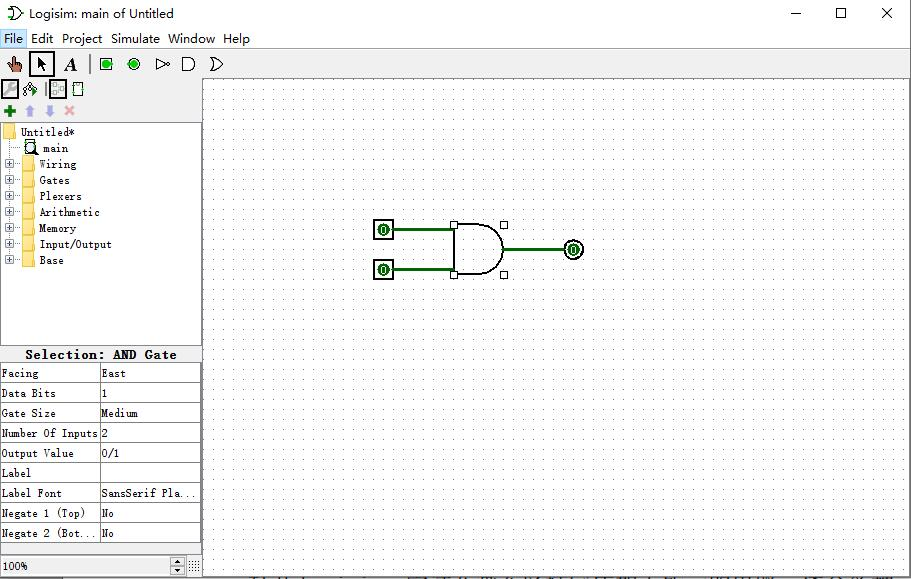
\includegraphics[scale=0.4]{layout.jpg}
		\caption{Logisim的界面布局}
		\label{layout}
	\end{figure}
	\subsection{熟悉Logisim基本操作}
	通过练习,了解:按钮、 LED、输入管脚、输出管脚、多位宽信号、探针、分线器、基本逻辑门等各类组件,以及不同颜色的线缆所代表的含义。
	\subsection{模块封装}
	在 Logisim 软件中, 新建一个新的电路命名为“Add” ,并绘制电路结构, 完成半加器的设计\par
%	\begin{figure}[!h]
%		\centering
%		\begin{minipage}[h]{0.45\linewidth}
%			\centering
%			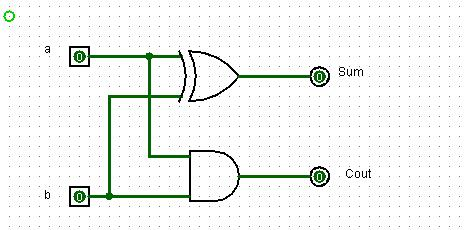
\includegraphics[width=1\textwidth]{detail_of_half-adder.jpg}
%			\caption{封装半加器}
%		\end{minipage}
%		\begin{minipage}[h]{0.45\linewidth}
%			\centering
%			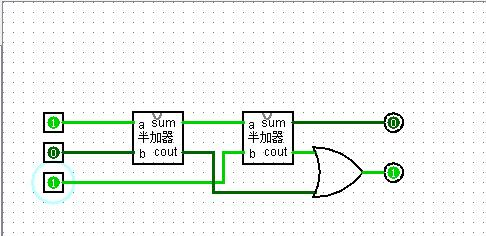
\includegraphics[width=1\textwidth]{use_of_half-adder.jpg}
%			\caption{封装的半加器的使用}
%		\end{minipage}
%	\end{figure}
	
	\begin{figure}[H]
		\centering
		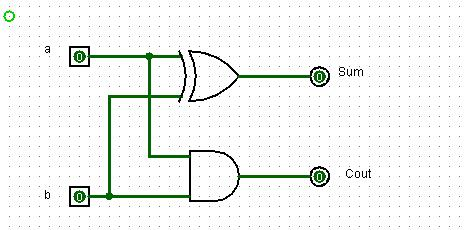
\includegraphics[scale=0.4]{detail_of_half-adder.jpg}
		\caption{封装半加器}
		\label{detailofhalfadder}
	\end{figure}
	
	\begin{figure}[H]
		\centering
		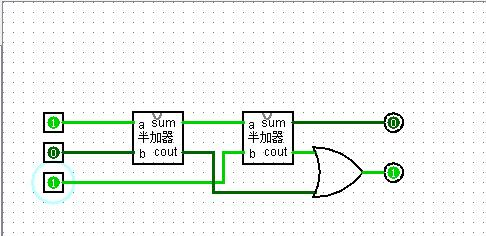
\includegraphics[scale=0.4]{use_of_half-adder.jpg}
		\caption{封装的半加器的使用}
		\label{useofhalfadder}
	\end{figure}
	
	\section{实验练习}
	
	\subsection{题目1}
	\subsubsection{题目}
	使用合适分辨率的 LED 点阵显示出自己的姓名。\par
	\subsubsection{实验结果}
	实验结果如下图所示:
	\begin{figure}[h]
		\centering
		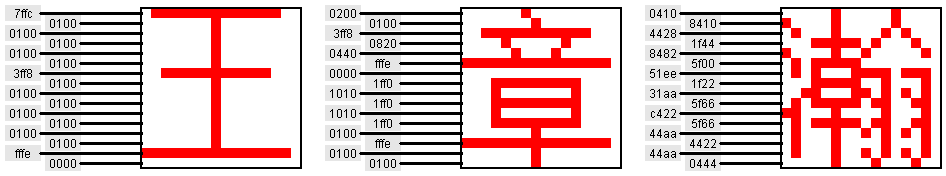
\includegraphics[scale=0.4]{1.png}
		\caption{题目1实验结果}
		\label{1}
	\end{figure}

	
	\subsection{题目2}
	\subsubsection{题目}
	请用若干个共阴极七段数码管显示出自己的学号。\par
	\subsubsection{实验结果}
	实验结果如下图所示:
	\begin{figure}[H]
		\centering
		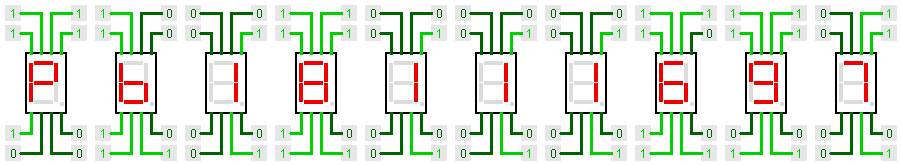
\includegraphics[scale=0.4]{2.png}
		\caption{题目2实验结果}
		\label{2}
	\end{figure}
	
	\subsection{题目3}
	\subsubsection{题目}
	如下图所示,是用晶体管搭出来的三个逻辑门,试分析其行为特性,判定各自为哪种逻辑门。 \par
	\subsubsection{实验结果}
	经分析,各个逻辑门的行为特性所对应的逻辑门类型均已标注在下图。\par
	实验结果如下图所示:
	\begin{figure}[H]
		\centering
		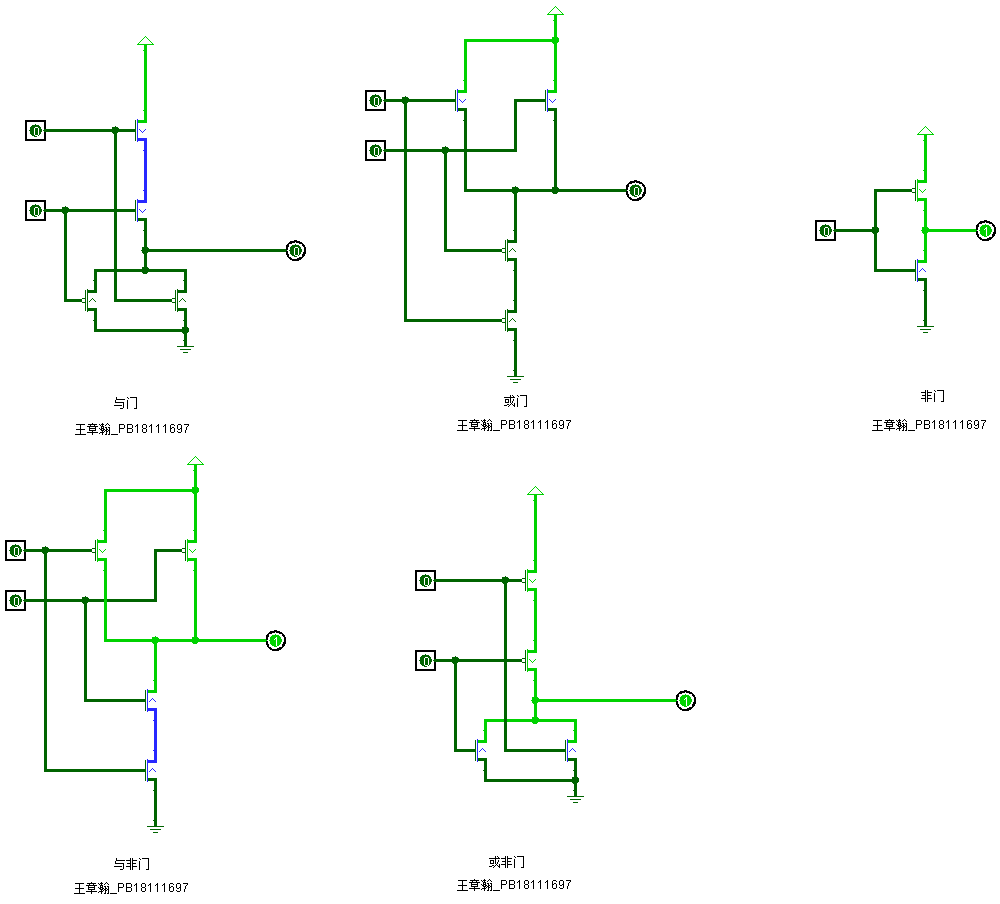
\includegraphics[scale=0.25]{3.png}
		\caption{题目3实验结果}
		\label{3}
	\end{figure}
	
	\subsection{题目4}
	\subsubsection{题目}
	将前面设计的单 bit 与门、或门、非门进行封装,并使用自己搭建的三种基本门电路设计一个 1bit 位宽的二选一选择器,统计各种基本门的数量。如设计一个 2bit位宽的四选一选择器,三种基本门各需要多少个?\par
	\subsubsection{实验结果}
	按如下图所示的设计:\par
	一个1bit位宽的二选一选择器,需要与门2个,或门1个,非门1个;\par
	一个2bit位宽的四选一选择器,需要与门12个,或门6个,非门4个。\par
	实验结果如下图所示:
	\begin{figure}[H]
		\centering
		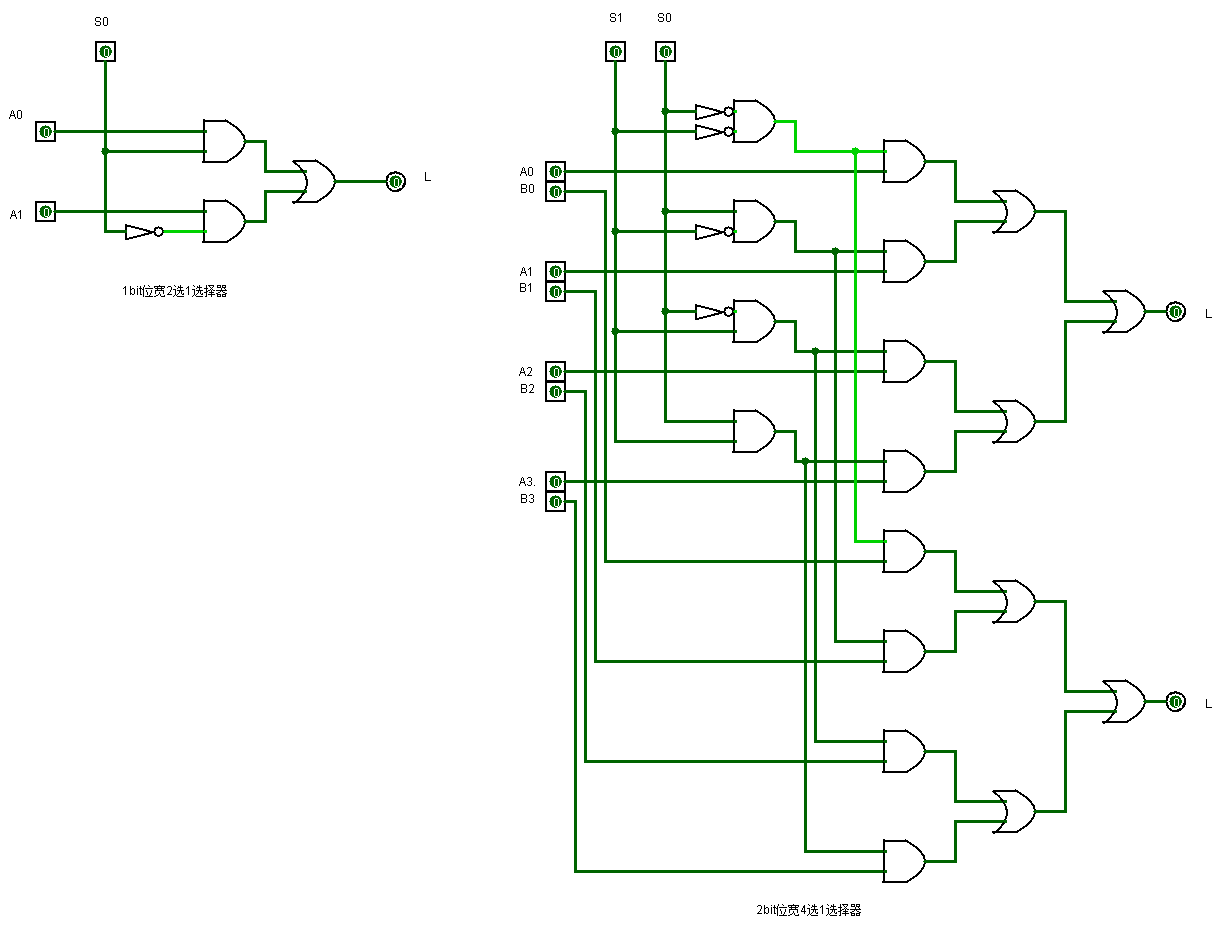
\includegraphics[scale=0.3]{4.png}
		\caption{题目4实验结果}
		\label{4}
	\end{figure}
	
	\section{总结与思考}
	
	\subsection{本次实验的收获}
	在本次实验中,我初步了解了Logisim的界面布局与操作。能够使用Logisim中的各个功能,包括使用各种组件,设置组件参数,了解各种颜色线的含义,能够自己封装电路等。\par
	
	\subsection{评价本次实验的难易程度}
	本次实验内容相对简单,能够只依靠实验指导书来完成实验内容,而不需要自己查询资料。\par
	
	\subsection{评价本次实验的任务量}
	本次实验任务量适中,虽然需要花2到3小时的时间,但相对合理。\par
	
	\subsection{为本次实验提供改进建议}
	本次实验的实验指导书详实,通俗易懂,暂无其他建议。
	
\end{document}
